% Where in the spectrum each method's error sits: the relative error of every one
% of the first 1000 eigenvalues against its index, at one moderate resolution,
% one series of markers per discretisation. L-shaped domain, logarithmic index.
%
% The same data as L_shaped_error_distribution_n1000_dofs2241.tex, whose index
% axis is linear. Neither shows what the other does: the linear axis gives the
% body of the block the room it deserves, most of the thousand eigenvalues living
% in the last decade, and it is there that FD and FEM separate and rejoin; this
% one opens out the first few indices, which the linear axis presses against the
% left edge. That is where the ordering of the three methods is the reverse of
% what it is everywhere else -- at the ground state DST is the worst of them and
% FEM the best, the re-entrant corner costing DST more than it costs the others,
% and by the top of the block DST is three orders of magnitude ahead.
%
% Markers and no connecting lines: the quantity is one number per eigenvalue, and
% neighbouring indices belong to unrelated eigenfunctions, so a line through them
% would invite a trend to be read through what is a scatter of separate results.
%
% The DST series is drawn in two parts. The L-shape is three unit squares, and
% the eigenfunctions vanishing on the two internal edges are the square's own,
% with eigenvalue pi^2*(m^2+n^2) known in closed form; on the bounding box those
% are sine modes of even index, so the DST operator carries them exactly and
% returns their eigenvalues at any resolution. There are 326 of them in the first
% thousand, every one reproduced at 2241 degrees of freedom to within 4.3e-12
% relative and with the right multiplicity. Drawn together with the rest they
% swamp them, so they are the filled dots and the remaining indices the open
% circles. FD and FEM have no such subspace and are drawn whole.
%
% The split is decided on the run and the reference together, not on the
% reference alone. The two spectra are sorted ascending and compared index by
% index, and at six of the 326 a neighbouring eigenvalue -- one DST resolves only
% to about 1e-4 -- crosses the exact one in the ordering, so that the run's k-th
% entry is a different eigenvalue from the reference's. The value plotted there
% is a genuine mismatch between unlike eigenvalues and has nothing to do with how
% well DST returns the exact ones, so those six are drawn as open circles. The
% filled population is then exactly the set of indices at which DST returned the
% eigenvalue the reference has.
%
% The reference is a DST run at M = 163, 19845 degrees of freedom, the L-shape
% having no closed-form spectrum and no published values away from the ground
% state. What it is worth is not uniform across the figure, and this is the
% figure where that matters most: at low index run and reference are both DST and
% share whatever the re-entrant corner does to them, so the DST markers at the
% left-hand edge are an upper bound on its accuracy rather than a measured error.
% The FD and FEM series, orders of magnitude larger over most of the block, are
% unaffected.
%
% Requires in the preamble:
%   \usepackage{graphicx}
%   \usepackage{epstopdf}   % the figure is EPS; needed under pdflatex,
%                           % which then wants -shell-escape. Not needed for
%                           % latex/dvips, which reads EPS directly.
%
% The figure lives next to this file, in results_paper/eigenvalues_error_distribution/.
% If you \input this snippet from elsewhere, point graphicx at that folder, e.g.
%   \graphicspath{{results_paper/eigenvalues_error_distribution/}}
% and drop the leading path from the \includegraphics argument below.

\begin{figure}[htbp]
  \centering
  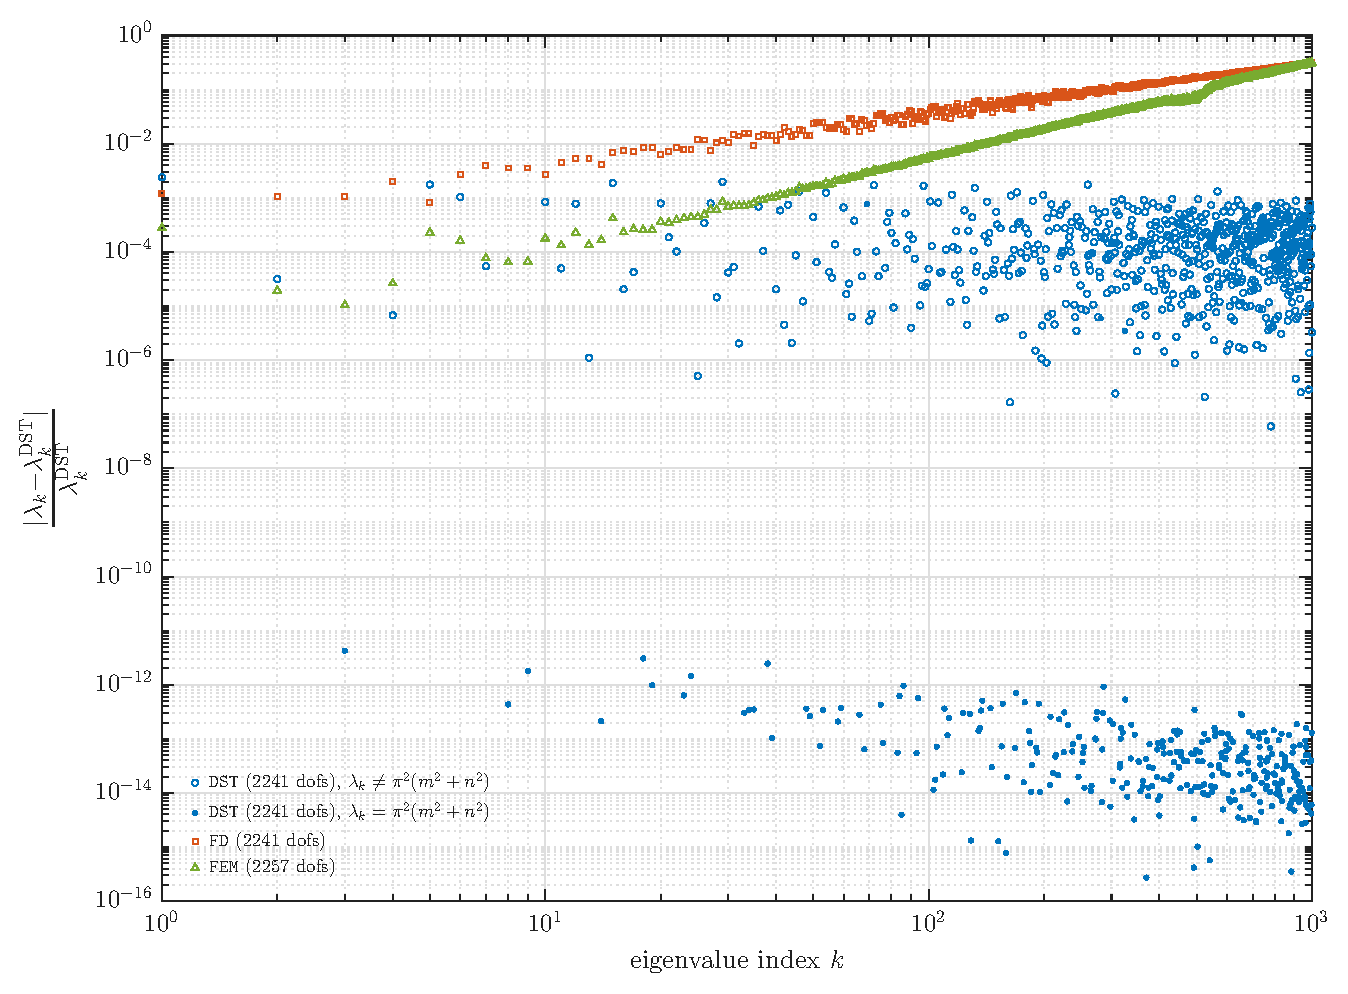
\includegraphics[width=0.85\textwidth]{L_shaped_error_distribution_n1000_dofs2241_log_log}
  \caption{Accuracy of the first 1000 eigenvalues of Laplace operator, zero Dirichlet boundary conditions, L-shaped domain \texttt{L\_shaped}, logarithmic eigenvalue index. Relative error $\frac{|\lambda_k - \lambda_k^{\text{DST}}|}{\lambda_k^{\text{DST}}}$ of each eigenvalue against its index $k$, $k = 1, \dots, 1000$, for three discretisations of Laplace operator at comparable numbers of degrees of freedom -- \texttt{DST} and \texttt{FD} 2241, \texttt{FEM} 2257 -- compared with the reference eigenvalues computed by \texttt{DST} with 19845 degrees of freedom. The \texttt{DST} series is split into the indices at which \texttt{DST} returns the eigenvalue $\lambda_k = \pi^2(m^2+n^2)$ of the three unit squares exactly, drawn as filled dots, and the remaining indices, drawn as open circles.}
  \label{fig:error_distribution_L_shaped_log_log}
\end{figure}
